\section{Generierung der Proxies auf Basis von Matchern}\label{sec_proxygen}
Ein \emph{Proxy} ist ein Objekt, das stellvertretend für ein anderes Objekt verwendet wird und den Zugang - in diesem Fall den Methodenaufruf - auf dieses Objekt kontrolliert (vgl. \cite{patterns}). Dadurch ist es dem \emph{Proxy} möglich, die Methodenaufrufe an andere Objekte zu delegieren. Diese Eigenschaft wird sich in dieser Arbeit zunutze gemacht, um einen Aufruf einer Methode, die in einem Typ (\emph{required} oder \emph{provided Typ}) deklariert wurde, an eine Methode zu delegieren, die in einem anderen \emph{provided Typ} deklariert wurde.
\\\\
Dabei wird zwischen einem \emph{Source-Typen} und einem oder mehrerer \emph{Target-Typen} unterschieden. Als \emph{Source-Typ} wird immer der Typ bezeichnet, für den der \emph{Proxy} generiert und stellvertretend eingesetzt wird. Bei den \emph{Target-Typen} handelt es sich um die \emph{provided Typen} an deren Methoden die Methodenaufrufe delegiert werden.
\\\\
Zur Beschreibung der Generierung von \emph{Proxies} wird im Folgenden zuerst vorgegeben, wie sich ein \emph{Proxy} deklarieren lässt. Darauf aufbauend werden die Generatoren, die in Abhängigkeit des Matchings zwischen \emph{Source-} und \emph{Target-Typen} Anwendung finden, beschrieben.
\subsection{Struktur für die Definition von Proxies}\label{sec:proxygram}
Die Grammatikregeln für die Deklaration eines \emph{Proxies} sind Tabelle \ref{tab:grProxies} zu entnehmen. Es handelt sich dabei um Produktionsregeln einer \Gls{attributgrammatik}. Die dazugehörigen Attribute sind der Tabelle \ref{tab:attrGrProxies} zu entnehmen. Dazu sei zusätzlich festgelegt, dass die Notation $\mathit{NT}\texttt{.}\text{*}$ in der Spalte \emph{Attribute} eine Key-Value-Liste aller Attribute des Nonterminals $\mathit{NT}$ beschreibt, wobei der Attributname als Key und dessen Wert als Value innerhalb der Liste verwendet wird. Weiterhin sei ein Attribut, dass in der Spalte \emph{Attribute} zu einem Nonterminal nicht aufgeführt ist, mit dem Wert \emph{none} belegt.
\newpage
\begin{table}[H]
\centering
\begin{tabular}{|p{5cm}|p{9cm}|}
\hline
\hline
\centering\textbf{Regel} & \textbf{Erläuterung} \\
\hline
\hline
$\mathit{PROXY} ::=$\newline
$\texttt{proxy } \texttt{for } T$\newline
$ \texttt{with [}\mathit{P_1},...,\mathit{P_n}\texttt{]}$ \newline
$\texttt{\{}\mathit{MDEL_1},...,\mathit{MDEL_k} \texttt{\}}$
 & Ein \emph{Proxy} wird für ein Typ $T$ als \emph{Source-Typ} mit einer Menge von \emph{provided Typen} $P = \{P_1,...,P_n\}$ als \emph{Target-Typen}, einer Menge von Methoden-Delegationen erzeugt.\\
\hline
$\mathit{MDEL} ::=$\newline
$CALLM \rightarrow DELM $  & Eine \emph{Methodendelegation} besteht aus einer \emph{aufgerufenen Methode} und aus einem \emph{Delegationsziel}.\\
\hline
$\mathit{CALLM} ::=$\newline 
$\mathit{REF}.\mathit{m(\mathit{CP_1},...,\mathit{CP_n}):CR} $  & Eine \emph{aufgerufene Methode} besteht aus dem Namen der Methode $m$, dem Rückgabetyp $\mathit{CR}$ und einer Menge von Parametertypen $\{\mathit{CP_1},...,\mathit{CP_n}\}$.\\
\hline
$\mathit{DELM} ::=$\newline 
$\mathit{REF}.\mathit{n(\mathit{DP_1},...,\mathit{DP_n}):DR} $  
& Die erste Variante eines \emph{Delegationsziels} besteht aus  dem Namen der \emph{Delegationsmethode} $n$, dem Rückgabetyp $\mathit{DR}$ und einer Menge von Parametertypen $\{\mathit{DP_1},...,\mathit{DP_n}\}$.\\
\hline
$\mathit{DELM} ::=$\newline
$\texttt{posModi(} \mathit{I_1},...,\mathit{I_n} \texttt{)}$\newline
$\mathit{REF}.\mathit{n(\mathit{DP_1},...,\mathit{DP_n}):DR} $  
& Die zweite Variante eines \emph{Delegationsziels} besteht aus einer Menge von Indizies $\{\mathit{I_1},...,\mathit{I_n}\}$, einer \emph{Referenz}, dem Namen der \emph{Delegationsmethode} $n$, dem Rückgabetyp $\mathit{DR}$ und einer Menge von Parametertypen $\{\mathit{DP_1},...,\mathit{DP_n}\}$.\\
\hline
$\mathit{DELM} ::= \texttt{err} $  
& Die dritte Variante eines \emph{Delegationsziels} enthält keine weiteren Bestandteile. Das Terminal $\texttt{err}$ weist darauf hin, dass die Delegation innerhalb des Proxies nicht möglich ist und zu einem Fehler führt.\\
\hline
$\mathit{REF} ::= \mathit{P_i}$
& Die erste Variante einer \emph{Referenz} besteht aus einem Typ $P_i$ .\\
\hline
$\mathit{REF} ::= \mathit{P_i}\texttt{.}\mathit{f}$
& Die zweite Variante einer \emph{Referenz} besteht aus einem Typ $P_i$ und einem Feldnamen $f$.\\
\hline
\end{tabular}
\caption{Grammatikregeln mit Erläuterungen für die Deklaration eines Proxies}
 \label{tab:grProxies}
\end{table}
\noindent
\begin{table}[H]
\centering
\begin{tabular}{|p{6cm}|p{10cm}|}
\hline
\hline
\centering\textbf{Regel} & \textbf{Attribute} \\
\hline
\hline
$\mathit{PROXY} ::=$\newline
$\texttt{proxy } \texttt{for } T$\newline
$ \texttt{with [}\mathit{P_1},...,\mathit{P_n}\texttt{]}$ \newline
$\texttt{\{}\mathit{MDEL_1},...,\mathit{MDEL_k} \texttt{\}}$
& 
$\texttt{type} = \mathit{T}$\newline
$\texttt{targets} = [\mathit{P_1},...,\mathit{P_n}]$\newline
$\texttt{dels} = [\mathit{MDEL_1}\texttt{.}\text{*},...,\mathit{MDEL_k}\texttt{.}\text{*}]$\newline
$\mathit{MDEL_1}\texttt{.call.field} = ... = \mathit{MDEL_k}\texttt{.call.field}$\newline
$\mathit{MDEL_1}\texttt{.del.field} = ... = \mathit{MDEL_k}\texttt{.del.field}$
\\
\hline
$\mathit{MDEL} ::=$\newline
$\mathit{CALLM} \rightarrow \mathit{DELM} $  
& 
$\texttt{call} = \mathit{CALLM}.*$\newline
$\texttt{del} = \mathit{DELM}.*$
\\
\hline
$\mathit{CALLM} ::=$\newline 
$\mathit{REF}.\mathit{m(\mathit{CP_1},...,\mathit{CP_n}):CR}$
& 
$\texttt{source} = \mathit{REF.\texttt{mainType}}$\newline
$\texttt{delType} = \mathit{REF.\texttt{delType}}$\newline
$\texttt{name} = \mathit{m}$\newline
$\texttt{paramTypes} = \mathit{[CP_1},...,\mathit{CP_n]}$\newline
$\texttt{returnType} = \mathit{CR}$\newline
$\texttt{field} = \mathit{REF}\texttt{.field}$\newline
$\texttt{paramCount} = n$
\\
\hline
$\mathit{DELM} ::=$\newline 
$\mathit{REF}\texttt{.}n(\mathit{DP_1},...,\mathit{DP_n}):DR $  
&
$\texttt{target} = \mathit{REF}.\texttt{mainType}$\newline
$\texttt{delType} = \mathit{REF}.\texttt{delType}$\newline
$\texttt{posModi} = [0,...,\mathit{n}-1]$\newline
$\texttt{name} = \mathit{n}$\newline
$\texttt{paramTypes} = \mathit{[DP_1},...,\mathit{DP_n]}$\newline
$\texttt{returnType} = \mathit{DR}$\newline
$\texttt{field} = \mathit{REF}\texttt{.field}$
\\
\hline
$\mathit{DELM} ::=\texttt{posModi(} \mathit{I_1},...,\mathit{I_n} \texttt{)}$\newline
$\mathit{REF}\texttt{.}n(\mathit{DP_1},...,\mathit{DP_n}):DR $  
&
$\texttt{target} = \mathit{REF}.\texttt{mainType}$\newline
$\texttt{delType} = \mathit{REF}.\texttt{delType}$\newline
$\texttt{posModi} = \mathit{[I_1},...,\mathit{I_n]}$\newline
$\texttt{name} = \mathit{n}$\newline
$\texttt{paramTypes} = \mathit{[DP_1},...,\mathit{DP_n]}$\newline
$\texttt{returnType} = \mathit{DR}$\newline
$\texttt{field} = \mathit{REF}\texttt{.field}$
\\
\hline
$\mathit{DELM} ::= \texttt{err} $  
&
\\
\hline
$\mathit{REF} ::= \mathit{P}$
& 
$\texttt{mainType} = \mathit{P}$\newline
$\texttt{field} = \texttt{self}$\newline
$\texttt{delType} = \mathit{P}$
\\
\hline
$\mathit{REF} ::= \mathit{P}\texttt{.}\mathit{f}$
&
$\texttt{mainType} = \mathit{P}$\newline
$\texttt{field} = \mathit{f}$\newline
$\texttt{delType} = \mathit{memType(f,P)}$
\\
\hline
\end{tabular}
\caption{Grammatikregeln mit Attributen für die Deklaration eines Proxies}
 \label{tab:attrGrProxies}
\end{table}
\noindent
\subsection{Delegation von Methoden im Proxy}
Ein \emph{Proxy} bietet alle Methoden des \emph{Source-Typen} an. Einige dieser Methoden werden an eine Methode delegiert, die von einem \emph{Target-Typ} des \emph{Proxies} angeboten wird. Eine solche Delegation wird durch eine \emph{Methoden-Delegation} (siehe Tabelle \ref{tab:attrGrProxies} Nontermial $\mathit{MDEL}$) definiert.
\begin{example}{bsp_methDel}
So beschreibt die folgende \emph{Methoden-Delegation}, dass die Methode $\texttt{extinguishFire}$, die vom \emph{Source-Typ} $\texttt{Patient}$ - und damit auch vom \emph{Proxy} - angeboten wird, an die Methoden $\texttt{heal}$, die der \emph{Target-Typ} $\texttt{Injured}$ anbietet, delegiert wird.
\begin{lstlisting}[style = dsl, caption = Einfache Methoden-Delegation, captionpos = b]
	Patient.heal(Medicine):void --> Injured.heal(Medicine):void
\end{lstlisting}
\end{example}
Die Delegation einer \emph{aufgerufenen Methode} an ein \emph{Delegationsziel}, erfolgt in drei Schritten.
\begin{enumerate}
\item Parameterübergabe\\
Dabei werden die Parameter, mit denen die vom \emph{Proxy} angebotene Methode aufgerufen wird, an die \emph{Delegationsmethode} des \emph{Delegationsziels} übergeben. Dabei sind zwei Dinge zu beachten. Zum einen müssen die Typen der übergebenen Parameter zu den Typen der von der \emph{Delegationsmethode} erwarteten Parameter passen. Zum anderen muss die Reihenfolge, in der die Parameter übergeben wurden, an die erwartete Reihenfolge der \emph{Delegationsmethode} angepasst werden. (siehe auch Funktion $\mathit{matchingParams}$ aus Abschnitt \ref{subsec_structmatcher})
\item Ausführung\\
Dieser Schritt meint die Durchführung der \emph{Delegationsmethode} mit den übergeben Parametern aus Schritt 1. Dies schließt auch die Ermittlung des korrekten Rückgabewertes der \emph{Delegationsmethode} ein.
\item Übergabe des Rückgabewertes\\
Ähnlich wie bei der Parameterübergabe, muss auch der Rückgabewert, der bei der Ausführung in Schritt 2 ermittelt wurde, an die \emph{aufgerufene Methode}, die vom \emph{Proxy} angeboten wird, übergeben werden. Hier muss ebenfalls sichergestellt werden, dass die beiden Rückgabetypen der beiden Methoden zueinander passen.
\end{enumerate}
Die Delegation aus dem oben genannten Beispiel kann schematisch wie in Abbildung \ref{fig:DEL_heal} dargestellt werden. Die Übergabe der Parameter- und Rückgabewerte wird durch die gestrichelten Pfeile symbolisiert.
\begin{figure}[h!]
\centering
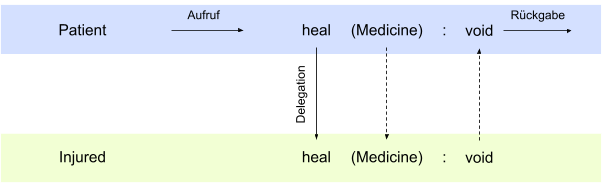
\includegraphics[width=1\linewidth]{MDEL_heal}
\caption{Delegation der Methode $\texttt{heal}$}
\label{fig:DEL_heal}
\end{figure}
\noindent
\\\\
In diesem Beispiel sind sowohl die Parameter- als auch die Rückgabe-Typen der \emph{aufgerufenen Methode} und der \emph{Delegationsmethode} identisch. Weiterhin spielt die Reihenfolge der Parameter in diesem Beispiel keine Rolle, da es nur einen Parameter gibt. Daher stellt die Übergabe der Parameter- und Rückgabewerte kein Problem dar.
\\\\
Folgendes Beispiel soll zeigen, wie mit unterschiedlichen Reihenfolgen bzgl. der Parameter bei einer \emph{Methoden-Delegation} umzugehen ist.

\begin{example}{bsp_methDel_posModi}
Die \emph{Methoden-Delegation} aus Listing \ref{lst:methdel2} ist ein Beispiel für einen solchen Fall. Hier wird die \emph{aufgerufene Methode} $\texttt{heal}$ mit den Parametern $\texttt{Patient}$ und $\texttt{MedCabinet}$ aus dem Typ $\texttt{PatientMedicalFireFighter}$ an die gleichnamige Methode aus dem Typ $\texttt{InverseDoctor}$ delegiert. Die \emph{Delegationsmethode} verwendet zwar identische Parameter-Typen, aber die Reihenfolge, in der die Parameter übergeben werden, ist unterschiedlich.
\begin{lstlisting}[style = dsl, caption = Methoden-Delegation mit Parametern in unterschiedlicher Reihenfolge, captionpos = b]
	PatientMedicalFireFighter.heal(Patient, MedCabinet):void --> posModi(1,0)  InverseDoctor.heal(MedCabinet,Patient):void
\end{lstlisting}\label{lst:methdel2}
\end{example}
Um die Reihenfolge der Parameter aus dem ursprünglichen Aufruf zu variieren, wird das Schlüsselwort $\texttt{posModi}$ verwendet. Dort werden eine Reihe von Indizes angegeben. Die Anzahl der angegebenen Indizes muss mit der Anzahl der Parameter übereinstimmen. Ein Index beschreibt die Position des in der \emph{aufgerufenen Methode} angegebenen Parameter. Weiterhin spielt die Reihenfolge der Indizes eine wichtige Rolle. Diese ist mit der Reihenfolge der Parameter der \emph{Delegationsmethoden} gleichzusetzen.
\\\\
So wird in dem o.g. Beispiel der erste Parameter der \emph{aufgerufenen Methoden} (Index = 0) der \emph{Delegationsmethode} als zweiter Parameter übergeben. Dementsprechend wird der zweite Parameter der \emph{aufgerufenen Methode} (Index = 1) der \emph{Delegationsmethode} als erster Parameter übergeben (siehe Abbildung \ref{fig:DEL_healInverse}). 
\begin{figure}[H]
\centering
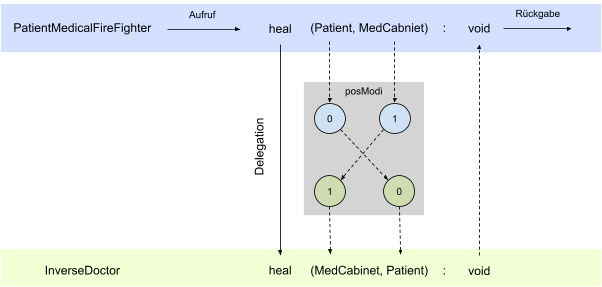
\includegraphics[width=1\linewidth]{MDEL_healInverse}
\caption{Delegation der Methode $\texttt{heal}$ mit Parametern in unterschiedlicher Reihenfolge}
\label{fig:DEL_healInverse}
\end{figure}
\noindent
\\
Dass identische Typen keine Probleme bei der Übergabe zwischen \emph{aufgerufener Methode} und \emph{Delegationsmethode} darstellen, wurde in den oben genannten Beispielen gezeigt.
Darüber hinaus können Typen aber auch dann ohne Probleme übergeben werden, wenn sie sich aufgrund des \Gls{substitutionsprinzip}s austauschen lassen. Daher kann ein Typ $T$ anstelle eines Typs $T'$ verwendet werden, sofern $T \leq T'$ gilt.
\\\\
Folgendes Beispiel soll zeigen, wie mit übergebenen Typen umzugehen ist, die nicht ohne Probleme übergeben werden können.

\begin{example}{bsp_methDel_proxy}
In folgendem Listing ist eine \emph{Methoden-Delegation} aufgerührt, bei der sowohl die Parameter- als auch die Rückgabe-Typen der \emph{aufgerufenen Methode} und der \emph{Delegationsmethode} nicht auf Basis des \Gls{substitutionsprinzip}s übergeben werden können.
\begin{lstlisting}[style = dsl, caption = Methoden-Delegation mit Typkonvertierung, captionpos = b, label = lst:methdel3 ]
	MedicalFireFighter.extinguishFire(ExtFire):boolean --> FireFigher.extinguishFire(Fire):FireState
\end{lstlisting}
\end{example}
In einem solchen Fall müssen die Parameter-Typen der \emph{aufgerufenen Methoden} in die Parameter-Typen der \emph{Delegationsmethode} konvertiert werden. Analog dazu muss der Rückgabetyp der \emph{Delegationsmethode} in den Rückgabetyp der \emph{aufgerufenen Methoden} konvertiert werden. Die Konvertierung wird dabei über die Generierung eines \emph{Proxies} erzielt.
\\\\
Angenommen, eine Funktion $\mathit{proxies(S,TM)}$ beschreibt eine Menge von \emph{Proxies}, mit $S$ als \emph{Source-Typ} und $\mathit{TM}$ als Menge der \emph{Target-Typen}, dann müssten bezogen auf die \emph{Methoden-Delegation} aus Listing \ref{lst:methdel3} für die Parameter einer der \emph{Proxies} aus $\mathit{proxies(\texttt{Fire}, \{\texttt{ExtFire}\})}$ an die \emph{Delegationsmethode} übergeben werden. Nach der Ausführung der \emph{Delegationsmethode} müsste aus dem Rückgabewert ein \emph{Proxy} aus $\mathit{proxies(\texttt{boolean},\{\texttt{FireState}\})}$ erzeugt werden und an die \emph{aufgerufene Methode} als Rückgabewert übergeben werden. Der Sachverhalt wird in Abbildung \ref{fig:DEL_extinguishFire} schematisch dargestellt. Die grauen Kästen symbolisieren die Generierung eines Proxies. Wie die \emph{Proxies} generiert werden, wird im folgenden Abschnitt beschrieben.
\newpage
\begin{figure}[H]
\centering
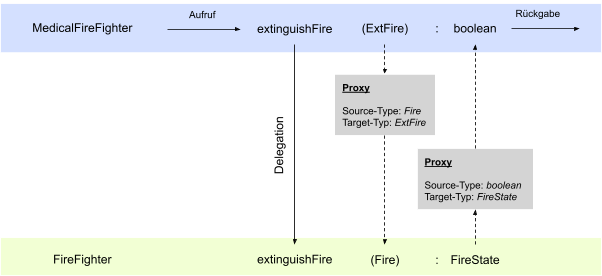
\includegraphics[width=1\linewidth]{MDEL_extinguishFire}
\caption{Delegation der Methode $\texttt{extinguishFire}$ mit Typkonvertierungen}
\label{fig:DEL_extinguishFire}
\end{figure}
\noindent


\subsection{Generierung von Proxies}\label{sec_proxyGen}
Wie im Abschnitt \ref{sec:proxygram} bereits angedeutet, soll die Menge der \emph{Proxies} für einen \emph{Source-Typ} $S$ und einer Menge von \emph{Target-Typen} $\mathit{TM}$ über die Funktion $\mathit{proxies(S,\mathit{TM})}$ beschrieben werden.
\\\\
In Abhängigkeit von dem Matching zwischen dem \emph{Source-Typ} und den \emph{Target-Typen} werden unterschiedliche Arten von \emph{Proxies} generiert. Für die unterschiedlichen \emph{Proxy}-Arten gibt es ebenfalls Funktionen, die eine Menge von \emph{Proxies} zu einem \emph{Source-Typen} $S$ und einer Menge von \emph{Target-Typen} $\mathit{TM}$ beschreiben.
\\\\
In den folgenden Abschnitten werden diese Funktionen für die einzelnen Proxy-Arten beschrieben. Dabei ist davon auszugehen, dass die \emph{Proxies} eine allgemeine Struktur haben, die in Abschnitt \ref{sec:proxygram} aufgeführt ist. Um die Regeln für die Generierung der \emph{Proxies} zu beschreiben, soll davon ausgegangen werden, dass jedes Listen-Attribut ($\mathit{NT.}\text{*}$) aus Tabelle \ref{tab:attrGrProxies} ein Attribut $\texttt{len}$ enthält in dem die Anzahl der Elemente abgelegt ist, die sich in dieser Liste befinden.


\subsubsection{Sub-Proxy}
Die Voraussetzung für die Erzeugung eines \emph{Sub-Proxies} vom Typ $S$ (\emph{Source-Typ}) aus einem \emph{Target-Typ} $\mathit{T}$ ist $S \Rightarrow_{spec} T$. Damit ist der \emph{SpecTypeMatcher} der \emph{Basis-Matcher} für den \emph{Sub-Proxy}.

\begin{example}{bsp_subproxy}
Als Beispiel soll  der Typ $\texttt{Patient}$ als \emph{Source-Typ} und der Typ $\texttt{Injured}$ als \emph{Target-Typ} verwendet werden. Da $\texttt{Patient} \Rightarrow_{spec} \texttt{Injured}$ gilt, kann ein \emph{Sub-Proxy} für diese Konstellation erzeugt werden. Der resultierende \emph{Sub-Proxy} ist in Listing \ref{lst:subproxy} aufgeführt. Der abstrakte Syntaxbaum (\acrshort{ast}) mit den dazugehörigen Attributen ist Abbildung \ref{fig:ASTSUB} zu entnehmen. \footnote{Es wurden nur die Nonterminale mit den dazugehörigen Attributen aufgeführt.}
\begin{lstlisting}[style = dsl, caption = Sub-Proxy für Patient, captionpos = b, label = lst:subproxy]
proxy for Patient with [Injured]{
	Patient.heal(Medicine):void --> Injured.heal(Medicine):void
	Patient.getName():String --> err
}
\end{lstlisting}
\end{example}
Ein \emph{Proxy} bietet alle Methoden an, die auch von dessen \emph{Source-Typ} angeboten werden. Sofern für eine angebotene Methode keine \emph{Methodendelegationen} innerhalb des \emph{Proxies} existiert, wird diese Methode so ausgeführt, wie sie innerhalb des \emph{Source-Typen} implementiert wurde. Anderenfalls beschreiben die \emph{Methodendelegationen} innerhalb eines \emph{Proxies}, was beim Aufruf der entsprechenden Methode passiert. So wird ein Aufruf der Methode $\texttt{heal}$ an die Methode $\texttt{heal}$ aus dem \emph{Target-Typ} delegiert. Ein Aufruf der Methode $\texttt{getName}$ hingegen führt zu einem Fehler, weil keine passende \emph{Delegationsmethode} zur Verfügung steht.
\\\\
Weiterhin beschreibt der \emph{Sub-Proxy} aus dem Beispiel auch, dass der Aufruf der Methode $\texttt{getName}$ zu einem Fehlschlag führt. Dies ist auf eine Problematik zurückzuführen, die auch bei einem \Gls{downcast} auftritt. Hierbei soll ein Objekt eines Super-Typs anstelle eines Objektes eines Sub-Typs verwendet werden. Das Objekt des Sub-Typs bietet jedoch mitunter Methoden an, die im Super-Typ nicht deklariert wurden. Folglich können diese Methoden nicht ausgeführt werden, was jedoch häufig erst zur Laufzeit auffällt.
\begin{figure}[H]
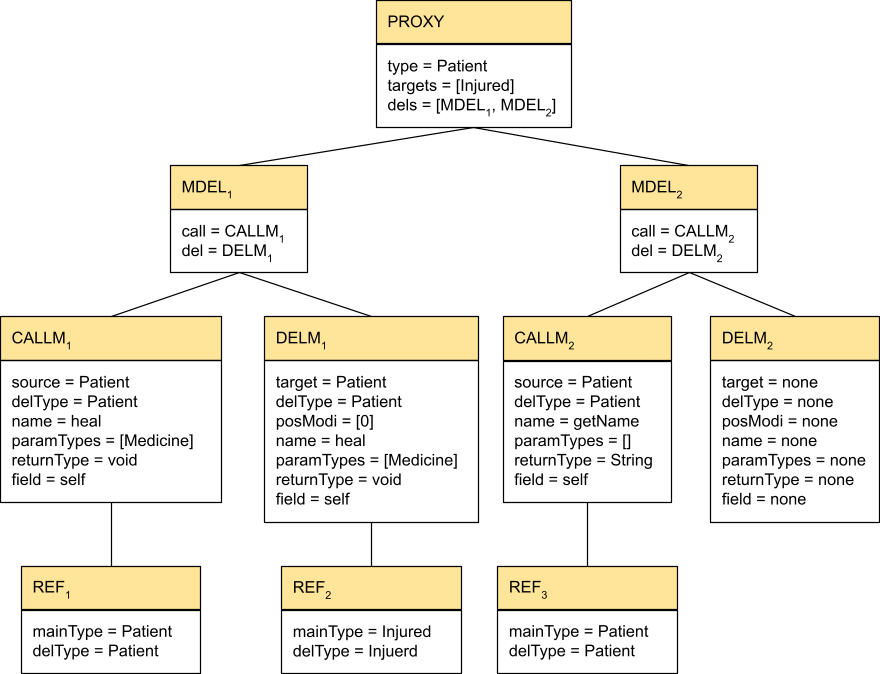
\includegraphics[width=\linewidth]{AST_SubExample}
\caption{AST für das Beispiel zum Sub-Proxy}
\label{fig:ASTSUB}
\end{figure}
\paragraph{Formalisierung}
Formal wird ein \emph{Sub-Proxy} für einen \emph{Source-Typ} $S$ auf der Basis von einer Menge von \emph{Target-Typen} $\mathit{TM}$ durch die Regeln beschrieben, die im Folgenden vorgestellt werden.
\\\\
Ein \emph{Sub-Proxy} enthält genau einen \emph{Target-Typ}. Für einen \emph{Proxy} $P$ wird dieser Sachverhalt durch die folgende Regel dargestellt.
\begin{gather*}
\frac{|\mathit{P.targets}| = 1 \wedge \forall \mathit{T} \in \mathit{TM}: T \in \mathit{P.targets}}{\mathit{targets_{single}(P,\mathit{TM})}}
\end{gather*}
\noindent
Darüber hinaus kann für jeden \emph{Proxy} $P$ (egal welcher Art) festgehalten werden, dass dessen Attribut $\texttt{type}$ immer mit einem bestimmten Typen $S$ übereinstimmt. Damit wird ausgesagt, dass $S$ der \emph{Source-Typ} des \emph{Proxies} $P$ ist.
\begin{gather*}
\frac{\mathit{P.type} = \mathit{S}}{\mathit{proxy(P,S)}}
\end{gather*}
\noindent
Die Unterschiede der einzelnen Proxy-Arten lassen sich in den \emph{Methoden-Delegationen} finden. Eine \emph{Methoden-Delegationen} besteht aus einer linken Seite - die \emph{aufgerufene Methode} - und eines rechten Seite - die \emph{Delegationsmethode}. Bevor die Beziehungen zwischen diesen beiden Seiten beschrieben werden, werden zuerst die separaten Eigenschaften der beiden Seiten beschrieben.
\\\\
So muss die \emph{aufgerufene Methode} immer im Typ aus dem Attribut $\texttt{call.delType}$ deklariert sein.
\begin{gather*}
\frac{\exists \mathit{T'\text{ } m(T)} \in \mathit{methods(MD.call.delType)}: \mathit{MD.call.name} = m}
{\mathit{callDecl(MD)}}
\end{gather*}
\noindent
Bezüglich des Feldes $\texttt{delType}$ der \emph{Delegationsmethode} gilt ähnliches.
\begin{gather*}
\frac{\exists \mathit{T'\text{ }m(T)} \in \mathit{methods(MD.del.delType)}: \mathit{MD.del.name} = m}
{\mathit{delDecl(MD)}}
\end{gather*}
\noindent
Darüber hinaus müssen die Attribute $\texttt{source}$ und $\texttt{delType}$ der \emph{aufgerufenen Methode} einer \emph{Methoden-Delegation} $\mathit{MD}$ mit dem \emph{Source-Typ} des \emph{Proxies} belegt sein. Dazu müssen die beiden folgenden Regeln gelten.
\begin{gather*}
\frac{\mathit{MD.call.source} = \mathit{MD.call.delType}}
{\mathit{callDelegationType_{simple}(MD)}}
\end{gather*}
\begin{gather*}
\frac{\mathit{MD.call.source} = \mathit{P.type}}
{\mathit{sourceType(MD, P)}}
\end{gather*}
\noindent
Damit ist auch automatisch gewährleistet, dass das Attribut $\texttt{field}$ im Attribut $\texttt{call}$ der \emph{Methoden-Delegation} mit dem Wert $\texttt{self}$ belegt ist (vgl. Tabelle \ref{tab:attrGrProxies}).
\\\\
Ähnliches gilt für die Attribute $\texttt{field}$ und $\texttt{mainType}$ im Attribut $\texttt{del}$ der \emph{Methoden-Delegation} $\mathit{MD}$. Hierbei muss der Wert des Attributs $\texttt{mainType}$ jedoch mit dem \emph{Target-Typ} des \emph{Proxies} übereinstimmen.
\begin{gather*}
\frac{\mathit{MD.del.target} \in \mathit{P.targets} }
{\mathit{targetType(MD, P)}}
\end{gather*}
\begin{gather*}
\frac{\mathit{MD.del.delType} = \mathit{MD.del.target} }
{\mathit{delDelegationType_{sub}(MD)}}
\end{gather*}
Damit ist wiederum automatisch gewährleistet, dass das Attribut $\texttt{field}$ im Attribut $\texttt{del}$ der \emph{Methoden-Delegation} mit dem Wert $\texttt{self}$ belegt ist (vgl. Tabelle \ref{tab:attrGrProxies}).
\\\\
Die Regeln für die linke Seite einer \emph{Methoden-Delegation} $\mathit{MD}$ innerhalb eines \emph{Proxies} $P$ können damit in folgender Regel zusammengefasst werden:
\begin{gather*}
\frac{\mathit{callDecl(MD)} \wedge \mathit{callDelegationType_{simple}(MD,P)} \wedge \mathit{sourceType(MD,P)}}
{\mathit{call_{simple}(MD,P)}}
\end{gather*}
Dementsprechend dazu können auch die Regeln für die rechte Seite einer \emph{Methoden-Delegation} $\mathit{MD}$ innerhalb eines \emph{Proxies} $P$ zusammengefasst werden:
\begin{gather*}
\frac{\mathit{delDecl(MD)} \wedge \mathit{targetType_{sub}(MD,P) \wedge \mathit{delDelegationType_{sub}(MD)}}}
{\mathit{del_{simple}(MD,P)}}
\end{gather*}
\noindent
Die oben genannten Regeln beschreiben die notwendigen Bedingungen der beiden Seiten einer \emph{Methoden-Delegation} innerhalb eines \emph{Sub-Proxies}. Die Bedingungen, die für eine gesamte \emph{Methoden-Delegation} $\mathit{MD}$ eines \emph{Sub-Proxies} $P$ gilt, werden durch die folgenden beiden Regeln beschrieben.
\begin{gather*}
\frac{\mathit{MD.call.name} = \mathit{MD.del.name}}
{\mathit{methodMatch_{simple}(MD)}}
\end{gather*}
\begin{gather*}
\frac{\mathit{call_{simple}(MD, P)} \wedge \mathit{del_{simple}(MD, P)} \wedge \mathit{methodMatch_{simple}}}
{\mathit{delegation_{sub}(MD, P)}}
\end{gather*}
\noindent
Zu beachten ist jedoch, dass ein \emph{Sub-Proxy} $P$ auch fehlschlagende \emph{Methoden-Delegationen} $\mathit{MD}$ enthalten kann. Somit gilt ebenfalls:
\begin{gather*}
\frac{ \mathit{MD.del.name} = \texttt{none}}
{\mathit{methodErr(MD)}}
\end{gather*}
\begin{gather*}
\frac{\mathit{call_{simple}(MD, P)} \wedge \mathit{methodErr(MD)}}
{\mathit{delegation_{sub}(MD, P)}}
\end{gather*}
\noindent
Die Regel für alle \emph{Methoden-Delegationen} eines \emph{Sub-Proxies} $P$ lässt sich aufbauend auf den oben genannten Regeln, wie folgt darstellen.
\begin{gather*}
\frac{\forall \mathit{MD} \in P.dels: \mathit{delegation_{sub}(MD,P)}}
{\mathit{delegations_{sub}(P)}}
\end{gather*}
\noindent
Die Menge der \emph{Sub-Proxies}, die mit dem \emph{Source-Typ} $S$ und der Menge von \emph{Target-Typen} $\mathit{TM}$ erzeugt werden, wird darauf aufbauend durch die folgende Funktion beschrieben.
\begin{gather*}
\mathit{proxies_{sub}(S,\mathit{TM})} := 
\left\{\begin{array}{l|l}
		& \mathit{proxy(P,S)}\wedge \mathit{ } \\
	P	& \mathit{targets_{single}(P,\mathit{TM})} \wedge \mathit{ } \\
		& \mathit{delegations_{sub}(P)}
		 \end{array}
\right\}
\end{gather*}
\subsubsection{Content-Proxy}
Die Voraussetzung für die Erzeugung eines \emph{Content-Proxies} vom Typ $S$ aus einem \emph{Target-Typ} $T$ ist $S \Rightarrow_{content} T$. Damit ist der \emph{ContentTypeMatcher} der Basis-Matcher für den \emph{Content-Proxy}.

\begin{example}{bsp_contentproxy}
Als Beispiel sollen die Typen $\texttt{Medicine}$ und $\texttt{MedCabinet}$ verwendet werden, welche ein Matching der Form $\texttt{Medicine} \Rightarrow_{content} \texttt{MedCabinet}$ aufweisen. Daher kann ein \emph{Content-Proxy} für diese Konstellation erzeugt werden. Ein resultierender \emph{Content-Proxy} ist in folgendem Listing aufgeführt.
\newpage
\begin{lstlisting}[style = dsl, caption = Content-Proxy für Medicine, captionpos = b]
proxy for Medicine with [MedCabinet]{
	Medicine.getDesciption():String --> MedCabinet.med.getDesciption():String
}
\end{lstlisting}
Durch die Methoden-Delegation dieses \emph{Content-Proxies} wird die Methode $\texttt{getDescription}$ an das Feld $\texttt{med}$ des \emph{Target-Typen} $\texttt{MedCabniet}$ delegiert.\\\\
Der \acrshort{ast} mit den dazugehörigen Attributen ist Abbildung \ref{fig:ASTCONTENT} zu entnehmen. \footnote{Es wurden nur die Nonterminale mit den dazugehörigen Attributen aufgeführt.}

\end{example}
\begin{figure}[h!]
\centering
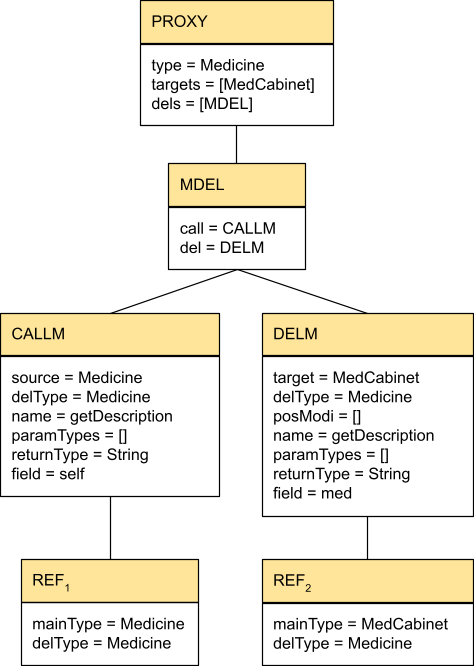
\includegraphics[width=0.5\linewidth]{AST_ContentExample}
\caption{AST für das Beispiel zum Content-Proxy}
\label{fig:ASTCONTENT}
\end{figure}
\paragraph{Formalisierung}
Formal wird ein \emph{Content-Proxy} durch die Regeln beschrieben, die im Folgenden vorgestellt werden.\\\\
Ein \emph{Content-Proxy} enthält, wie auch der \emph{Sub-Proxy}, genau einen \emph{Target-Typ}. Ebenfalls identisch zum \emph{Sub-Proxy} sind die Bedingungen hinsichtlich der \emph{aufgerufenen Methoden} in den einzelnen \emph{Methoden-Delegationen}.
\\\\
In den \emph{Delegationsmethoden} einer einzelnen \emph{Methoden-Delegation} $\mathit{MD}$ muss zwar ebenfalls das Attribut $\texttt{target}$ in den \emph{Target-Typen}  des \emph{Proxies} $P$ enthalten sein ($\mathit{targetType(MD,P}$), allerdings muss im \emph{Content-Proxy} darüber hinaus jenes Attribut $\texttt{target}$ ein Matching zum Typen im Attribut $\texttt{delType}$ aufweisen. 
\begin{gather*}
\frac{\mathit{P.type} \Rightarrow_{internCont} \mathit{MD.del.delType}}
{\mathit{delDelegationType_{content}(MD,P)}}
\end{gather*}
\noindent
Folglich werden auch die Eigenschaften einer \emph{Delegationsmethode} in einer \emph{Methoden-Delegation} $\mathit{MD}$ im \emph{Content-Proxy} durch eine andere Regel beschrieben als beim \emph{Sub-Proxy}:
\begin{gather*}
\frac{\mathit{delDecl(MD)} \wedge \mathit{targetType(MD,P) \wedge \mathit{delDelegationType_{content}(MD,P)}}}
{\mathit{del_{content}(MD,P)}}
\end{gather*}
\noindent
Darauf aufbauend ergibt sich wiederum folgende Regel für eine gesamte \emph{Methoden-Delegation} $\mathit{MD}$ innerhalb eines \emph{Content-Proxies} $P$.
\begin{gather*}
\frac{\mathit{call_{simple}(MD, P)} \wedge \mathit{del_{content}(MD, P)} \wedge \mathit{methodMatch_{simple}}}
{\mathit{delegation_{content}(MD, P)}}
\end{gather*}
\noindent
Da auch ein \emph{Content-Proxy} fehlschlagende \emph{Methoden-Delegationen} enthalten kann, muss ebenfalls gelten:
\begin{gather*}
\frac{\mathit{call_{simple}(MD, P)} \wedge \mathit{methodErr(MD)}}
{\mathit{delegation_{content}(MD, P)}}
\end{gather*}
\noindent
Für die Gesamtheit der \emph{Methoden-Delegationen} innerhalb eines \emph{Content-Proxies} $P$ muss dann gelten:
\begin{gather*}
\frac{\mathit{\forall \mathit{MD} \in P.dels: \mathit{delegation_{content}(MD,P)}}}
{\mathit{delegations_{content}(P)}}
\end{gather*}
\noindent
Die Menge der \emph{Content-Proxies}, die mit dem \emph{Source-Typ} $S$ und der Mengen von \emph{Target-Typen} $\mathit{TM}$ erzeugt werden, wird durch die folgende Funktion beschrieben.
\begin{gather*}
\mathit{proxies_{content}(S,\mathit{TM})} := 
\left\{\begin{array}{l|l}
		& \mathit{proxy(P,S)} \wedge \mathit{ } \\
	P	& \mathit{targets_{single}(P,\mathit{TM})} \wedge \mathit{ }\\
		& \mathit{delegations_{content}(P)} 
		 \end{array}
\right\}
\end{gather*}
\subsubsection{Container-Proxy}
Die Voraussetzung für die Erzeugung eines \emph{Container-Proxies} vom Typ $S$ aus einem \emph{Target-Typ} $T$ ist $S \Rightarrow_{container} T$. Damit ist der \emph{ContainerTypeMatcher} der Basis-Matcher für den \emph{Container-Proxy}.

\begin{example}{bsp_containerproxy}
Als Beispiel werden wiederum die Typen $\texttt{Medicine}$ und $\texttt{MedCabinet}$ verwendet, welche ein Matching der Form $\texttt{MedCabinet} \Rightarrow_{container} \texttt{Medicine}$ aufweisen. Daher kann ein \emph{Content-Proxy} für diese Konstellation erzeugt werden. Ein resultierender \emph{Content-Proxy} ist in folgendem Listing aufgeführt.
\begin{lstlisting}[style = dsl, caption = Container-Proxy für MedCabniet, captionpos = b ]
proxy for MedCabinet with [Medicine]{
	MedCabinet.med.getDesciption():String --> Medicine.getDesciption():String
}
\end{lstlisting}
Durch die \emph{Methoden-Delegation} dieses \emph{Container-Proxies} findet eine Delegation nur dann statt, wenn die Methoden $\texttt{getDescription}$ auf dem Feld $\texttt{med}$ des \emph{Source-Typ} aufgerufen wird. Diese wird dann an den \emph{Target-Typen} $\texttt{MedCabniet}$ delegiert.
\newpage
Der \acrshort{ast} mit den dazugehörigen Attributen ist Abbildung \ref{fig:ASTCONTAINER} zu entnehmen. \footnote{Es wurden nur die Nonterminale mit den dazugehörigen Attributen aufgeführt.}

\end{example}
\begin{figure}[h!]
\centering
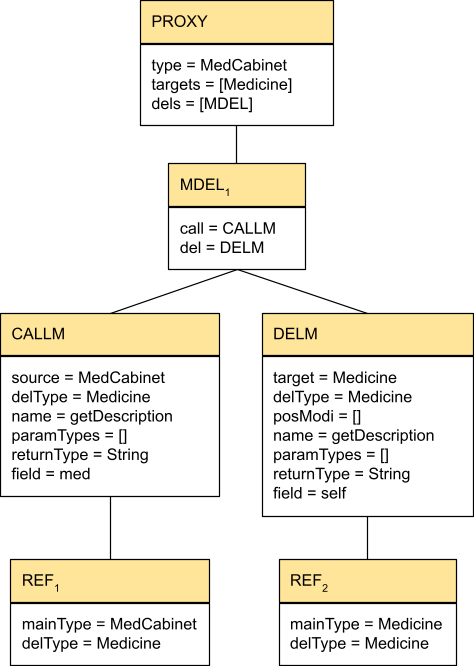
\includegraphics[width=0.5\linewidth]{AST_ContainerExample}
\caption{AST für das Beispiel zum Container-Proxy}
\label{fig:ASTCONTAINER}
\end{figure}
\noindent
\paragraph{Formalisierung}
Formal wird ein \emph{Container-Proxy} durch die Regeln beschrieben, die im Folgenden vorgestellt werden.
\\\\
Ein \emph{Container-Proxy} enthält, wie die vorher beschriebenen \emph{Proxies}, genau einen \emph{Target-Typ}. Die Eigenschaften der \emph{Delegationsmethoden} innerhalb der einzelnen \emph{Methoden-Delegationen} gleichen denen aus dem \emph{Sub-Proxy}.
\\\\
In der \emph{aufgerufenen Methode} einer einzelnen \emph{Methoden-Delegation} $\mathit{MD}$ muss das Attribut $\texttt{source}$ ebenfalls wie im \emph{Sub-Proxy} mit dem \emph{Source-Typen} des \emph{Proxies} $P$ übereinstimmen ($\mathit{sourceType(MD,P)}$), allerdings muss das Attribut $\texttt{delType}$ der \emph{aufgerufenen Methode} ein Matching zu einem der \emph{Target-Typen} des \emph{Proxies} aufweisen:
\begin{gather*}
\frac{\exists T \in \mathit{P.targets}:\mathit{MD.call.delType} \Rightarrow_{internCont} T}
{\mathit{callDelegationType_{container}(MD)}}
\end{gather*}
\noindent
Folglich werden auch die Eigenschaften einer \emph{aufgerufenen Methode} in einer \emph{Methoden-Delegation} $\mathit{MD}$ im \emph{Container-Proxy} durch eine andere Regel beschrieben als beim \emph{Sub-Proxy}:
\begin{gather*}
\frac{\mathit{callDecl(MD)} \wedge \mathit{callDelegationType_{container}(MD,P)} \wedge \mathit{sourceType(MD,P)}}
{\mathit{call_{container}(MD,P)}}
\end{gather*}
\noindent
Darauf aufbauend ergibt sich wiederum folgende Regel für eine gesamte \emph{Methoden-Delegation} $\mathit{MD}$ innerhalb eines \emph{Container-Proxies} $P$.
\begin{gather*}
\frac{\mathit{call_{container}(MD, P)} \wedge \mathit{del_{simple}(MD, P)} \wedge \mathit{methodMatch_{simple}}}
{\mathit{delegation_{container}(MD, P)}}
\end{gather*}
\noindent
Da auch ein \emph{Container-Proxy} fehlschlagende \emph{Methoden-Delegationen} enthalten kann, muss ebenfalls gelten:
\begin{gather*}
\frac{\mathit{call_{container}(MD, P)} \wedge \mathit{methodErr(MD)}}
{\mathit{delegation_{container}(MD, P)}}
\end{gather*}
\noindent
Für die Gesamtheit der \emph{Methoden-Delegationen} innerhalb eines \emph{Container-Proxies} $P$ muss dann gelten:
\begin{gather*}
\frac{\mathit{\forall \mathit{MD} \in P.dels: \mathit{delegation_{container}(MD,P)}}}
{\mathit{delegations_{container}(P)}}
\end{gather*}
\noindent
Die Menge der \emph{Container-Proxies}, die mit dem \emph{Source-Typ} $S$ und der Menge von \emph{Target-Typen} $\mathit{TM}$ erzeugt werden, wird durch die folgende Funktion beschrieben.
\begin{gather*}
\mathit{proxies_{container}(S,\mathit{TM})} := 
\left\{\begin{array}{l|l}
		& \mathit{proxy(P,S)}  \wedge \mathit{ } \\
	P	& \mathit{target_{single}(P,\mathit{TM})} \wedge \mathit{ } \\
		& \mathit{delegations_{container}(P)} 
		 \end{array}
\right\}
\end{gather*}
\subsubsection{Struktureller Proxy}\label{sssec_structproxy}
Die Voraussetzung für die Erzeugung eines \emph{strukturellen Proxies} vom \emph{required Typ} $R$ aus einem Target-Typ $T$ ist $R \Rightarrow_{struct} T$. Damit ist der \emph{StructuralTypeMatcher} der Basis-Matcher für den \emph{strukturellen Proxy}.
\\\\
Der \emph{strukturelle Proxy} ist der einzige \emph{Proxy}, der mit mehreren \emph{Target-Typen} erzeugt werden kann. 

\begin{example}{bsp_structproxy}
Als Beispiel werden die Typen $\texttt{MedicalFireFighter}$, $\texttt{Doctor}$ und $\texttt{FireFighter}$ verwendet. Dabei ist $\texttt{MedicalFireFighter}$ der \emph{Source-Typ} des \emph{Proxies} und die Menge der anderen beiden Typen bilden die \emph{Target-Typen} des \emph{Proxies}. Da der \emph{Source-Typ }zu den \emph{Target-Typen} ein Matching der Form $\texttt{MedicalFireFighter} \Rightarrow_{struct} \texttt{FireFighter}$ sowie\linebreak $\texttt{MedicalFireFighter} \Rightarrow_{struct} \texttt{Doctor}$ aufweist, kann ein \emph{struktureller Proxy} erzeugt werden. Ein solcher ist in folgendem Listing aufgeführt.
\begin{lstlisting}[style = dsl, caption = Struktureller Proxy für MedicalFireFighter, captionpos = b]
proxy for MedicalFireFighter with [Doctor, FireFighter]{
 MedicalFireFighter.heal(Patient, MedCabinet):void -->
    Doctor.heal(Patient, Medicine):void
 MedicalFireFighter.extinguishFire(ExtFire):boolean --> FireFighter.extinguishFire(Fire):FireState
}
\end{lstlisting}
In diesem Beispiel wird der Methodenaufruf der Methode $\texttt{heal}$ auf dem \emph{Proxy} an die Methode $\texttt{heal}$ des Typs $\texttt{Doctor}$ delegiert. Analog dazu würde ein Aufruf der Methode $\texttt{extinguishFire}$ auf dem Proxy an die Methode $\texttt{extinguishFire}$ des Typs $\texttt{FireFighter}$ delegiert werden. Die Methoden stimmen jeweils strukturell überein.
\\\\
Der \acrshort{ast} mit den dazugehörigen Attributen ist Abbildung \ref{fig:ASTSTRUCT} zu entnehmen. \footnote{Es wurden nur die Nonterminale mit den dazugehörigen Attributen aufgeführt.}

\end{example}
\begin{figure}[h!]
\centering
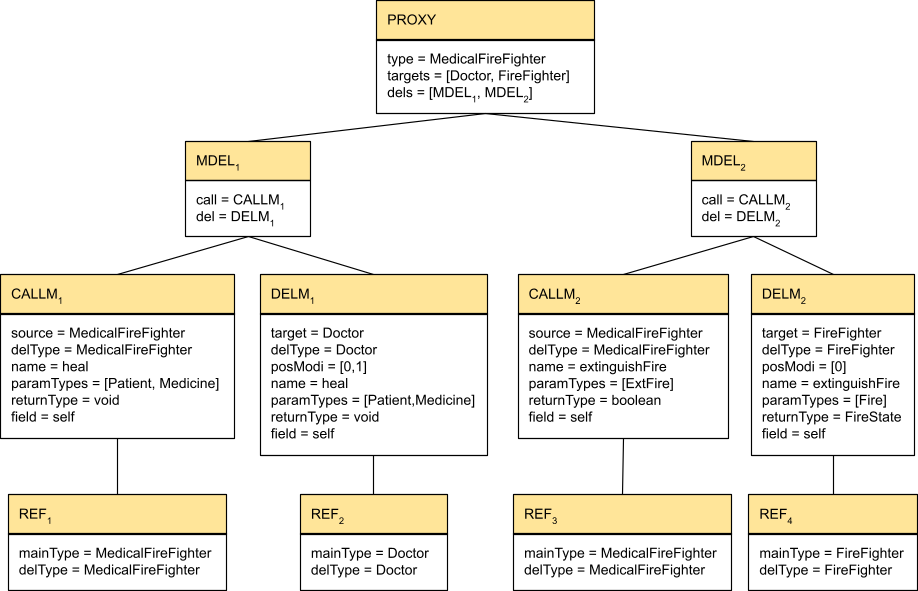
\includegraphics[width=\linewidth]{AST_StructExample}
\caption{AST für das Beispiel zum strukturellen Proxy}
\label{fig:ASTSTRUCT}
\end{figure}
\noindent
\paragraph{Formalisierung}
Ein \emph{struktureller Proxy} wird formal durch die folgenden Regeln beschrieben.
\\\\
Ein \emph{struktureller Proxy} kann, wie bereits erwähnt, mehrere \emph{Target-Typen} $\mathit{TM}$ enthalten.
Für jeden \emph{Target-Typ} $T \in \mathit{TM}$ muss dabei jedoch wenigstens eine \emph{Delegationsmethode} im \emph{Proxy} mit einem Attribut $\texttt{target} = T$ existieren. Dadurch gilt die für einen \emph{strukturellen Proxy} $P$:
\begin{gather*}
\frac{|\mathit{P.targets}| = |\mathit{TM}| \wedge \forall \mathit{T} \in \mathit{P.targets}: T \in \mathit{TM} \wedge \exists \mathit{MD} \in \mathit{P.dels}:\mathit{MD.del.target} = T}{\mathit{targets_{multi}(P, \mathit{TM})}}
\end{gather*}
\noindent
Für die \emph{aufgerufene Methode} und die \emph{Delegationsmethode} einer einzelnen \emph{Methoden-Delegation} gelten im \emph{strukturellen Proxy} dieselben Regeln wie für den \emph{Sub-Proxy}. Die Namen der \emph{aufgerufenen Methoden} und der \emph{Delegationsmethode} müssen dabei jedoch nicht übereinstimmen. Dafür müssen diese beiden Methoden jedoch ein strukturelles Matching aufweisen. Bezogen auf die Rückgabe-Typen einer \emph{aufgerufenen Methode} $\mathit{C}$ und einer \emph{Delegationsmethode} $\mathit{D}$ müssen daher folgende Regeln gelten.
\begin{gather*}
\frac{\mathit{D.returnType} \Rightarrow_{internStruct} \mathit{C.returnType}}{\mathit{returnMatch(C,D)}}
\end{gather*} 
\noindent
Weiterhin muss für die Parameter-Typen gelten:
\begin{gather*}
\frac{
\mathit{C.paramTypes}[i] \Rightarrow_{internStruct} \mathit{D.paramTypes}[\mathit{D.posModi}[i]]}{\mathit{posModiMatch(C,D,i)}}
\end{gather*} 
\begin{gather*}
\frac{\forall \mathit{i} \in \{0,...,\mathit{C.paramCount}-1\}: \mathit{posModiMatch(C,D,i)}
}{\mathit{paramsMatch(C,D)}}
\end{gather*} 
\noindent
Das strukturelle Matching zwischen einer einer \emph{aufgerufenen Methode} $C$ und einer \emph{Delegationsmethode} $D$ kann darauf aufbauend wie folgt beschrieben werden.
\begin{gather*}
\frac{\mathit{returnMatch(C,D) \wedge \mathit{paramsMatch(C,D)}}}
{\mathit{methodMatch_{struct}(C,D)}}
\end{gather*}
\noindent
Für eine einzelne \emph{Methoden-Delegation} $\mathit{MD}$ eines \emph{strukturellen Proxies} $P$ kann dann folgende Regel aufgestellt werden.
\begin{gather*}
\frac{\mathit{call_{simple}(MD, P)} \wedge \mathit{del_{simple}(MD, P)} \wedge \mathit{methodMatch_{struct}(MD.call, MD.del)}}
{\mathit{delegation_{struct}(MD, P)}}
\end{gather*}
\noindent
In einem \emph{strukturellen Proxy} muss für jede Methode $m$ des \emph{Source-Typen} genau eine \emph{Methoden-Delegation} mit der Methode $m$ als \emph{aufgerufene Methode} existieren:
\begin{gather*}
\frac{|\mathit{methods(P.type)}| = P.dels.len}{delegationCount_{struct}(P)}
\end{gather*}
\noindent
Für die Gesamtheit der \emph{Methoden-Delegationen} aus einem \emph{strukturellen Proxy} $P$ muss dann gelten:
\begin{gather*}
\frac{\mathit{delegationCount_{struct}(P)} \wedge \forall \mathit{MD} \in P.dels: \mathit{delegation_{struct}(MD,P)}}
{\mathit{delegations_{struct}(P)}}
\end{gather*}
\noindent
Die Menge der \emph{strukturellen Proxies}, die mit dem \emph{Source-Typ} $S$ und der Menge von \emph{Target-Typen} $\mathit{TM}$ erzeugt werden, wird aufbauend auf den oben genannten Regeln durch die folgende Funktion beschrieben.
\begin{gather*}
\mathit{proxies_{struct}(S,\mathit{TM})} := 
\left\{\begin{array}{l|l}
		& \mathit{proxy(P,S)}\wedge \mathit{ }\\
	P	& \mathit{targets_{multi}(P,\mathit{TM})} \wedge \mathit{ }\\
		& \mathit{delegations_{struct}(P)}  
		 \end{array}
\right\}
\end{gather*}

\subsubsection{Allgemeine Generierung von Proxies}
Die Proxy-Funktionen der einzelnen Proxy-Arten werden zur Beschreibung einer allgemeine Funktion für die Generierung der \emph{Proxies} verwendet. Dazu sind die Proxy-Arten zusammen mit den dazugehörigen \emph{Matchingrelationen} und den Namen der Funktionen zur Generierung des jeweiligen \emph{Proxies} in Tabelle \ref{tab:baseMatcher} noch einmal aufgeführt.

\begin{table}[H]
\centering
\begin{tabular}{|c|c|c|}
\hline
\hline
\centering\textbf{Proxy-Art} & \textbf{Matchingrelation} & \textbf{Funktionsname}\\
\hline
\hline
Sub-Proxy
&  
$\Rightarrow_{spec}$
& 
$\mathit{proxies_{sub}}$
\\
\hline
Content-Proxy
& 
$\Rightarrow_{content}$
& 
$\mathit{proxies_{content}}$
\\
\hline
Container-Proxy
& 
$\Rightarrow_{container}$
& 
$\mathit{proxies_{container}}$
\\
\hline
Struktureller Proxy
&
$\Rightarrow_{struct}$
& 
$\mathit{proxies_{struct}}$
 \\
\hline
\hline
\end{tabular}
\caption{Proxy-Arten mit Matchingrelationen und Proxy-Funktionen}
 \label{tab:baseMatcher}
\end{table}
\noindent
Die im Abschnitt \ref{sec:proxygram} erwähnte Funktion $\mathit{proxies(S,\mathit{TM})}$ kann darauf aufbauend für einen \emph{Source-Typ} $S$ und eine Menge von \emph{Target-Typen} $\mathit{TM}$ wie folgt beschrieben werden.
\begin{gather*}
\mathit{proxies(S,\mathit{TM})} := 
\left\{\begin{array}{ll}
\mathit{proxies_{sub}(S,\mathit{TM})}	& \text{wenn } |\mathit{TM}| = 1 \wedge \mathit{ }\\
& \forall T \in \mathit{TM}: S \Rightarrow_{spec} T\\	
&\\
\mathit{proxies_{content}(S,\mathit{TM})}	& \text{wenn } |\mathit{TM}| = 1 \wedge \mathit{ }\\
& \forall T \in \mathit{TM}: S \Rightarrow_{content} T \\
&\\
\mathit{proxies_{container}(S,\mathit{TM})} & \text{wenn } |\mathit{TM}| = 1 \wedge \mathit{ } \\
& \forall T \in \mathit{TM}: S \Rightarrow_{container} T \\
&\\
\mathit{proxies_{struct}(S,\mathit{TM})} & \text{wenn } |\mathit{TM}| > 0 \wedge \mathit{ } \\
&\forall T \in \mathit{TM}: S \Rightarrow_{struct} T
		 \end{array}
\right\}
\end{gather*}
\subsection{Anzahl struktureller Proxies innerhalb einer Bibliothek}\label{sec_anzahlProxies}
Die Generierung der \emph{strukturellen Proxies} für ein \emph{required Typ} $R$ aus der Bibliothek $L$ erfolgt während des \emph{Explorationsprozesses} auf Basis der Mengen von \emph{provided Typen} aus $\mathit{cover(R,L)}$ (siehe Abschnitt \ref{sec_ergStructEval}). Bezüglich dieser Mengen aus $\mathit{cover(R,L)}$ gilt jedoch folgendes Theorem\footnote{Der Beweis ist in Anhang \ref{app_proofs} zu finden.}:
\begin{theorem}\label{lemma_targetcount}
Sei $R$ ein \emph{required Typ} innerhalb einer Bibliothek $L$. 
Ein \emph{struktureller Proxy} für $R$ lässt sich nur aus den Mengen $\mathit{TM} \in \mathit{cover(R,L)}$ generieren, für die gilt:
\begin{gather*}
|\mathit{TM}| \leq |\mathit{methods(R)}|
\end{gather*}
\end{theorem}
\noindent
Mit einer Menge $\mathit{TM} \in \mathit{cover(R,L)}$, für die die Bedingung aus Theorem \ref{lemma_targetcount} eingehalten wird, können durchaus mehrere \emph{Proxies} erzeugt werden. Das ist dann der Fall, wenn mehrere der Methoden, die in den \emph{provided Typen} aus $\mathit{TM}$ deklariert wurden, mit einer Methode aus $R$ strukturell übereinstimmen, oder wenn für eine Methode $m$ aus $R$ und eine Methode $m'$ aus einem der \emph{Target-Typen} $|matchingParams(m,m')| > 1$ gilt (siehe Abschnitt \ref{subsec_structmatcher}).
\\\\
Die Anzahl der \emph{strukturellen Proxies} für einen \emph{required Typ} $R$ mit einer bestimmten Menge von \emph{Target-Typen} ist somit von der Anzahl der Methoden abhängig, die in einem der \emph{Target-Typen} deklariert wurden und strukturell mit den Methoden aus $R$ übereinstimmen. 
\\\\
Die Menge der Methoden eines \emph{provided Typs} $T$, die strukturell mit einer Methode $m$ übereinstimmen, wird über die Funktion $\mathit{structM_{target}}$ beschrieben.
\begin{gather*}
\mathit{structM_{target}(m, T)} := 
\left\{\begin{array}{l|l}
m'	& m' \in \mathit{methods(T)} \wedge  m \Rightarrow_{method} m'
\end{array}
\right\}
\end{gather*}
\noindent
Darauf aufbauend wird die Menge der Methoden einer Menge von \emph{provided Typen} $\mathit{TM}$, die strukturell mit einer Methode $m$ übereinstimmen, über die Funktion $\mathit{structM_{targetset}}$ beschrieben.
\begin{gather*}
\mathit{structM_{targetset}(m, \mathit{TM})} := 
\left\{\begin{array}{l|l}
m'	& \exists T \in \mathit{TM}: m' \in \mathit{structM_{target}(m,T)}
\end{array}
\right\}
\end{gather*}
\begin{example}{bsp_structmtarget}
Aufbauend auf dem Beispiel \ref{bsp_cover} ergeben sich für die Menge der \emph{Target-Typen}  $\{\texttt{Leave}, \texttt{Come}\}$ und die beiden Methoden des \emph{required Typs} $\texttt{Greeting}$ folgende Mengen von übereinstimmenden Methoden über die Funktion $\mathit{structM_{targetset}}$:
\begin{gather*}
\mathit{structM_{targetset}(\methodForm{String}{hello}{},\{\texttt{Leave}, \texttt{Come}\})} = 
\left\{
\begin{array}{l}
\methodForm{String}{hello}{},\\
\methodForm{String}{goodMorning}{},\\
\methodForm{String}{bye}{}
\end{array}
\right\}\\
\mathit{structM_{targetset}(\methodForm{String}{bye}{},\{\texttt{Leave}, \texttt{Come}\})} = 
\left\{
\begin{array}{l}
\methodForm{String}{hello}{},\\
\methodForm{String}{goodMorning}{},\\
\methodForm{String}{bye}{}
\end{array}
\right\}
\end{gather*}
\end{example}
Sei $R$ ein \emph{required Typ} und $\mathit{TM}$ eine Menge von \emph{provided Typen} innerhalb einer Bibliothek $L$ mit $\mathit{TM} \in \mathit{cover(R,L)}$. Dann bildet die Funktion $\mathit{structMSets}$ die Menge von Mengen der Methoden aus den Elementen aus $\mathit{TM}$ ab, die mit jeweils einer Methode aus $R$ gematcht werden können.
\newpage
\begin{gather*}
\mathit{structMSets(R,\mathit{TM})} := 
\left\{M
\begin{array}{l|l}
&\exists \mathit{m} \in \mathit{methods(R)} : 
\\
&M = \mathit{structM_{targetset}(m,\mathit{TM})}
\end{array}
\right\}
\end{gather*}
\noindent
Für die Bildung eines \emph{Proxies} wird aus jedem Element der Menge $structMSets(R,\mathit{TM})$ genau ein Element als \emph{Delegationsmethode} verwendet. 

\begin{example}{bsp_proxycreation}
Ausgehend von Beispiel \ref{bsp_structmtarget} lassen sich die folgenden vier \emph{Proxies} mit den \emph{Target-Typen} $\texttt{Leave}$ und $\texttt{Come}$ erzeugen.
\begin{lstlisting}[style = dsl]
proxy Greeting with [Come, Leave]{
 Greeting.hello():String --> Come.hello():String
 Greeting.bye():String --> Leave.bye():String
}
\end{lstlisting}
\begin{lstlisting}[style = dsl]
proxy Greeting with [Come, Leave]{
 Greeting.hello():String --> Come.goodMorning():String
 Greeting.bye():String --> Leave.bye():String
}
\end{lstlisting}
\begin{lstlisting}[style = dsl]
proxy Greeting with [Come, Leave]{
 Greeting.hello():String --> Leave.bye():String
 Greeting.bye():String --> Come.hello():String
}
\end{lstlisting}
\begin{lstlisting}[style = dsl]
proxy Greeting with [Come, Leave]{
 Greeting.hello():String --> Leave.bye():String
 Greeting.bye():String --> Come.goodMorning():String
}
\end{lstlisting}
\end{example}
\\
Die Anzahl aller möglichen \emph{strukturellen Proxies} für ein \emph{required Typ} $R$ aus einer Menge von \emph{Target-Typen} $\mathit{TM}$ sei näherungsweise über die Funktion $\mathit{proxyCount(R,\mathit{TM})}$ beschrieben. Dass es sich hierbei lediglich um eine Annäherung handelt liegt daran, dass eine Methode $\mathit{dm}$ mit $\mathit{dm} \in M_1 \cup ... \cup M_n$ und $\{M_1,...,M_n\} = \mathit{structMSets(R,TM)}$ innerhalb eines Proxy maximal einmal als \emph{Delegationsmethode} verwendet werden darf. Es ist jedoch möglich, dass es zwischen den Mengen 
$M_1,...,M_n$ Überschneidungen gibt (siehe vorheriges Beispiel). Darüber hinaus blenden die oben genannten Funktionen zur Ermittlung der matchenden Methoden die Anzahl der für die \emph{Methoden-Delegation} möglichen Parameter-Sortierungen aus $\mathit{matchtingParams}$ aus.
\\\\
Unter der Annahme, dass es nur eine mögliche Sortierung der Parameter für die matchenden Methoden gibt, gilt:
\begin{gather*}
\mathit{proxyCount(R,TM)} \leq 
\begin{array}{l|l}
\prod\limits_{i=1}^{n}|\mathit{structM_{targetset}(m_i, TM)}|
&
\left\{
\begin{array}{l}
m_1,\\
...,\\
m_n
\end{array}
\right\}
= \mathit{methods(R)}
\end{array}
\end{gather*}
\noindent
Durch mehrere Möglichkeiten der Sortierung der Parameter würde sich dieser Wert nochmals erhöhen. Auf eine genaue Formel wird an dieser Stelle verzichtet, da hier lediglich eine Vorstellung davon vermittelt werden soll, wie große die Anzahl der möglichen \emph{strukturellen Proxies} mit einer bestimmten Mengen von \emph{Target-Typen} ist.
\\\\
Da innerhalb einer Bibliothek $L$ mehrere Mengen von \emph{Target-Typen} zur Bildung eines \emph{Proxies} für einen \emph{required Typ} $R$ infrage kommen (siehe Funktion $\mathit{cover}$) muss die Anzahl der \emph{strukturellen Proxies} über die Funktion $\mathit{proxyCount}$ für alle Elemente aus $\mathit{cover(R,L)}$ ermittelt und summiert werden. Dabei muss jedoch beachtet werden, dass die Funktion $\mathit{cover}$ nicht die Bedingung aus Theorem \ref{lemma_targetcount} abbildet. Daher muss die Funktion für diesen Sachverhalt, wie folgt näherungsweise definiert werden:
\begin{gather*}
\mathit{libProxyCount(R,L)} \leq 
\begin{array}{l|l}
\sum_{i=1}^{n}\mathit{proxyCount(R,c_i)}
&
\left\{
\begin{array}{l}
c_1,\\
...,\\
c_n
\end{array}
\right\} = \mathit{cover(R,L)}
\end{array}
\end{gather*}